\section{Fujitsu}
\label{sec_fujitsu}

% vortragFujitsu
% Karsten Beins, Vortrag am Hasso-Plattner-Institut im Rahmen des Industrie-Seminars zum Cloud-Computing, 2014
%
% - Fujitsu
%	- führendes japanisches Unternehmen für Informations- und Kommunikationstechnik
%	- viertgrößter IT-Dienstleister der Welt
%	- Philosophie: Mensch im Mittelpunkt (Human-Centric Paradigm)
%		- Creativität, Flexibilität, Innovation...
% - Cloud
%	- hat sich von Hype zu Megatrend entwickelt 
%	-> Bild zu Gartner-Hype-Cycle 2014 (http://www.gartner.com/newsroom/id/2819918)
%		- sichtbar: diverse Cloud-Modelle erst in kommenden Jahren fruchtbar
% - Probleme mit Cloud
%	- aus technischer Sicht kein Problem (Modelle etc. mittlerweise vorhanden)
%	- für Business-Kunden: schwieriger Weg zur geeigneten Lösung
%	- Unternehmensapplikationen in die Cloud verschieben
%		- einfach und erprobt: einzelne Applikationen
%		- schwierig: eng miteinander vernetzte und komplexe Kernapplikationen
% - identifizierte Herausforderungen für Unternehmen, die Cloud verwenden wollen
%	- Datensicherheit: manche Daten müssen unter eigener Kontrolle bleiben (z.B. gesetzliche Regelungen)
%	- Datenschutz: werden Sicherheitsvorkehrungen vom Cloud-Anbieter umgesetzt? Gesetze wie der amerikanische Patriot-Act
%	- Kontrolle: wirksame Abgrenzung verschiedener Cloud-Kunden bei geteilter Infrastruktur
%	- Flexibilität: Entwicklung neuer Lösungen könnte mehr Flexibilität / Schutz erfordern, als für gewöhnlich möglich ist
%	- Komplexität
%		- Mehrzahl bestehender Applikationen nicht für Cloud ausgelegt
%		- komplexe Anwendungstopologien -> Deployment, Skalierung, Lifecycle Management, Migration zu / zwischen Cloud, Verfügbarkeit, Robustheit schwierig
%	- Integration: Interaktion zwischen Anwendungen in verschiedenen Clouds und klassischer IT-Infrastruktur
%	- Kosten: Voraussage der Kosten, vorteilhafte Applikationen
%	- Kenntnisse: Wissen erwerben, um mit diesen Herausforderungen umzugehen
% - Schlussfolgerungen (laut Vortrag)
%	- Abwägungen für Anwender, z.B.
%		- Servicemodell:
%			- Vereinfachung durch Abstraktion: PaaS, SaaS
%			- Flexibilität, feingranulare Kontrolle: IaaS
%		- Betriebsmodell:
%			- Preis, Skalierbarkeit: public clouds
%			- Datensicherheit, -schutz: on-premise / hosted private cloud

\IEEEPARstart{F}{ujitsu}\footnote{\url{http://www.fujitsu.com/}} ist das führende japanische Unternehmen für Informations- und Kommunikationstechnik und zudem der viertgrößte IT-Dienstleister der Welt. 

\subsection{Ansichten zu Cloud Computing}
\label{sec_fujitsu_general}

Im Folgenden werden die im Vortrag von Karsten Beins\cite{vortragFujitsu} dargelegten Ansichten zum Cloud Computing zusammengefasst.

Cloud Computing hat sich vom Hype zum Megatrend entwickelt. 
Wie im Gartner-Hype-Cycle von 2014, zu sehen in Abbildung \ref{fig:gartnerHypeCycle2014}, ersichtlich ist, befindet sich Cloud Computing im Allgemeinen auf dem Weg von Desillusionierung zu nützlicher Einsicht. 

\begin{figure*}
	\centering
	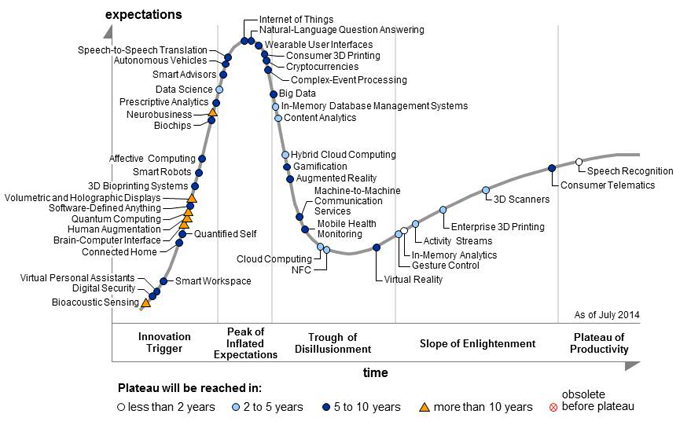
\includegraphics[width=0.8\linewidth]{images/gartnerHypeCycle2014}
	\caption{Gartner Hype Cycle 2014. http://www.gartner.com/newsroom/id/2819918, Zugriff 22.03.2015}
	\label{fig:gartnerHypeCycle2014}
\end{figure*}

\begin{description}
  \item[First] \hfill \\
  The first item
  \item[Second] \hfill \\
  The second item
  \item[Third] \hfill \\
  The third etc \ldots
\end{description}

\todo{mit SAP-Ansichten vergleichen}

\subsection{Service-Modelle}
\label{sec_fujitsu_delivery}



\subsection{Betriebsmodelle}
\label{sec_fujitsu_deployment}

